\chapter{ShallWeGo}
\newenvironment{code}{\captionsetup{type=listing}}{}

\begin{citazione}
    \textit{Lo scopo di questo capitolo è di descrivere in termini di implementazione il funzionamento e l'architettura della piattaforma. In particolare, si focalizza l'attenzione sulle tecnologie utilizzate per lo sviluppo del server e del client della piattaforma, oltre che ad altre tecnologie impiegate per il corretto funzionamento delle componenti.}
\end{citazione}

\newpage

\section{Requisiti funzionali}
    Allo scopo di questo lavoro di tesi, le seguenti funzionalità visibili all'utente sono state implementate:

    \begin{itemize}
        \item L'utente può visualizzare tramite una mappa le fermate dle trasporto pubblico presenti nin una determinata zona ed ottenerne i dettagli;
        \item Allo stesso modo, l'utente può visualizzare gli eventi temporanei in una determinata zona ed ottenerne i dettagli;
        \item L'utente può aggiungere delle fermate ad un elenco di fermate preferite;
        \item L'utente può visualizzare i dettagli e le destinazioni di una linea di trasporto pubblico;
        \item L'utente può seguire in diretta su una mappa l'andamento di una corsa e visualizzarne i dettagli;
        \item L'utente può segnalare l'affollamento di una fermata;
        \item L'utente può segnalare l'affollamento di una corsa;
        \item L'utente può segnalare la presenza di una fermata in un punto preciso sulla mappa o rapidamente presso la propria posizione;
        \item L'utente può segnalare la presenza di un'azienda di trasporto;
        \item L'utente può aggiungere una linea di trasporto pubblico ad un'azienda;
        \item L'utente può verificare, se gli sono state assegnate, tutti i tipi di segnalazioni appena descritti.
        \item L'utente può effettuare una segnalazione di un evento temporaneo in un punto preciso della mappa o rapidamente presso la propria posizione.
        \item L'utente può fornire aggiornamenti sulla propria posizione nell'ambito di una corsa espletata da una linea di trasporto pubblico e condividerne i dettagli.
    \end{itemize}

\section{Architettura del sistema}
    Il sistema ShallWeGo si configura come una classica architettura \textbf{client-server}.
    \begin{itemize}
        \item Il server consiste \textit{Java Enterprise application}, che accetta connessioni dal client sotto forma di richieste ad API REST.
        \item Il client è stato realizzato tramite un'applicazione utilizzabile sulla piattaforma Android dalla versione 10 in poi, a causa di scelte implementative riguardo alcune librerie incluse nel progetto. Queste scelte saranno documentate più avanti nel capitolo.
    \end{itemize}

    Per quanto riguarda la parte server, essa risulta composta da due macrocomponenti:

    \begin{itemize}
        \item La Java Application già accennata
        \item La componente che ospita la logica ed il database utilizzato da Nominatim, che è dislocato su un'altra macchina che viene utilizzata solo per questo scopo.
    \end{itemize}

\section{ShallWeGo: Il Server}
    Il server, come precedentemente menzionato, è realizzato usando le specifiche Java Enterprise Edition (da qui in poi \textit{Java EE}), usando a questo scopo il framework \textbf{\textit{Spring Boot}}, che permette una più semplice realizzazione dei task necessari a sviluppare un'applicazione che sfrutta il paradigma Client-Server, come ad esempio la gestione delle API accessibili dall'esterno i cosiddetti \textit{endpoint} oppure la gestione dei dati persistenti.

    \subsection{Class-Diagram}
        Di seguito è mostrato il diagramma delle classi del progetto Server. Sono state omesse le classi di servizio usate da Spring e da JPA per il corretto funzionamento del Server stesso. Sono inoltre state omesse le classi che compongono l'Algoritmo Genetico.

        \begin{figure}[H]
            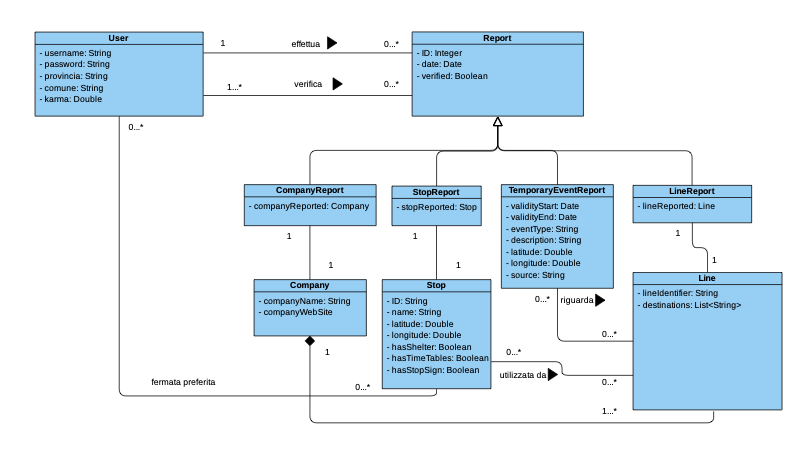
\includegraphics[width=\columnwidth]{ClassDiagram-cut}
            \caption{Il Class Diagram del Server}
            \label{fig: Il Class Diagram del Server}
        \end{figure}

    \subsection{Accessibilità delle API dall'esterno}
        Spring mette a disposizione il meccanismo dei \textbf{Controller}, che normalmente è inquadrato nel contesto di un'architettura MVC, anche se nel caso di ShallWeGo non vi è necessità di andare a creare un'applicazione di web che renda necessaria l'implementazione di tale pattern architetturale. Di conseguenza, essendo la parte che riguarda l'interfaccia utente gestita tramite un'applicazione Android, non è stata implementata nessuna parte che faccia le veci della "View" lato server. La comunicazione tra server e client avviene tramite JSON sfruttando il meccanismo delle API REST. La classe responsabile per la comunicazione con l'esterno è chiamata \textbf{Controller}, collocata nel pacchetto omonimo e decorati con l'annotazione \textbf{@RestController}. Questa annotazione permette al framework di interpretare quella classe come un Controller che accetta richieste sulla porta 8080 e all'indirizzo \url{/}. I vari metodi di quella classe che corrispondono alle diverse API esposte all'esterno sono decorati con una delle seguenti annotazioni:

        \begin{itemize}
            \item \textbf{@GetMapping("/url")} esegue il metodo annotato ogni qual volta all'indirizzo \url{/url} viene generata una richiesta di tipo \textbf{GET};
            \item \textbf{@PostMapping("/url")} esegue il metodo annotato ogni qual volta all'indirizzo \url{/url} viene generata una richiesta di tipo \textbf{POST};
            \item \textbf{@PutMapping("/url")} esegue il metodo annotato ogni qual volta all'indirizzo \url{/url} viene generata una richiesta di tipo \textbf{PUT};
            \item \textbf{@DeleteMapping("/url")} esegue il metodo annotato ogni qual volta all'indirizzo \url{/url} viene generata una richiesta di tipo \textbf{DELETE};
        \end{itemize}

    \subsection{Gestione dei dati persistenti: breve introduzione a JPA}
        Data la necessità di conservare una notevole quantità di dati (utenti, fermate, linee e così via) un approccio che prevede l'utilizzo di file è stato escluso a priori perché quasi impossibile da gestire data la complessità. Si è scelto quindi di utilizzare un database di tipo relazionale (RDBMS). Tuttavia, prevedendo il dominio applicativo numerose associazioni tra le entità, un approccio "classico" tramite \textbf{JDBC} avrebbe comunque portato ad un livello di complessità molto elevato (si pensi a dover gestire manualmente tutte le query con i vari join tra le tabelle). A questo scopo, torna molto utile sfruttare le caratteristiche di \textbf{ORM} (\textit{Object-Relational Mapping}) e, successivamente, di \textbf{JPA}, (\textit{Java Persistence API}).
        
        ORM è definito come "una tecnica di programmazione che permette l'integrazione di sistemi software che aderiscono al paradigma della programmazione orientata agli oggetti (\textbf{OOP}) con sistemi \textbf{RDBMS}".

        Uno dei principali vantaggi di ORM risiede nel contrasto della complessità di gestione della persistenza derivata dalla mancanza di compatibilità tra dati salvati all'interno di un database e oggetti in un linguaggio di programmazione, oltre che ad una sostanziale indipendenza dal \textit{vendor} che fornisce il DBMS utilizzato. \cite{wiki:orm}
        
        Il framework Spring, nello specifico, mette a disposizione una serie di API che implementano le specifiche di \textbf{JPA}. JPA è definito come "un insieme di specifiche che mette a disposizione degli sviluppatori un insieme di servizi e di strutture dati che permettono l'ORM e quindi la gestione dei dati persistenti all'interno di applicazioni Java." (\cite{jpa}). Essendo solamente una specifica, JPA necessita di un'implementazione. Quella di riferimento è \textbf{EclipseLink}, sviluppata dalla Eclipse Foundation a partire dal 2015.

        Il framework Spring, tuttavia, utilizza come implementazione delle specifiche JPA la libreria open source \textbf{Hibernate 5.5} sviluppata in partnership con l'azienda \textit{Red Hat}. 

        Per effettuare il mapping tra oggetti istanze di una classe e righe presenti in una tabella in un database, JPA si serve del concetto di \textbf{Entity}, che rappresenta un'istanza di una classe (in gergo, \textbf{POJO}, ovvero \textit{Plain Old Java Object}) che "dichiara" di poter essere salvata all'interno di un database.

        Le specifiche JPA introducono il concetto di \textbf{Configuration By Excpetion}. In questo modo, se non specificato altrimenti, le impostazioni riguardo persistenza e mapping di oggetti risulteranno essere quelle di default. Per fare un esempio concreto, in un progetto dove è previsto l'utilizzo di JPA tutte le classi Java vengono viste come tali fino a che non viene utilizzata l'annotazione Entity su una di queste. Ad esempio:

        \begin{code}
            \begin{minted}{java}
                @Entity
                public class POJO implements Serializable {
                    @Id 
                    private Integer id;

                    public POJO() {}
                }
            \end{minted}
            \caption{\textbf{File:} POJO.java}
        \end{code}
    
        Tramite questo setup è possibile rendere la classe contenuta in \textit{POJO.java} un'entity di cui è possibile effettuare la persistenza su un database.\\

        Per poter rappresentare un'Entity, un POJO deve rispettare i seguenti requisiti: (\cite{jee7})

        \begin{itemize}
            \item Essere annotata con \mintinline{java}{@javax.persistence.Entity};
            \item Avere un attributo annotato con \mintinline{java}{@javax.persistence.Id} che ne denota la chiave primaria (nel caso di chiave primaria semplice: è possibile anche avere chiavi composte, come descritto più avanti)
            \item Deve possedere un costruttore vuoto che abbia come modificatore di accesso \mintinline{java}{public} o \mintinline{java}{protected}. Sono ammessi ulteriori costruttori.
            \item Non deve essere una classe \textit{final}
            \item Non deve essere una classe interna ad un'altra classe
            \item Deve implementare l'interfaccia \mintinline{java}{Serializable}.
        \end{itemize}

        Le Entity presenti nel dominio applicativo sono le seguenti:

        \begin{itemize}
            \item \textbf{Stop}, che modella una fermata dei mezzi pubblici,
            \item \textbf{Line}, che modella una linea di trasporto pubblico,
            \item \textbf{Company}, che modella un'azienda di trasporto pubblico,
            \item \textbf{Report}, che modella il concetto di segnalazione,
            \item \textbf{LineReport}, che modella il concetto di segnalazione di una linea,
            \item \textbf{CompanyReport}, che modella il concetto di segnalazione di un'azienda,
            \item \textbf{StopReport}, che modella il concetto di segnalazione di una fermata,
            \item \textbf{TemporaryEventReport}, che modella il concetto di segnalazione di un evento temporaneo,
            \item \textbf{User}, che modella un utente registrato alla piattaforma.
        \end{itemize}

        oltre che ad altre classi "di servizio" create per mappare relazioni di tipo Many-to-Many.

        Si ponga attenzione sulla modellazione del concetto di segnalazione. Qui di seguito è mostrato lo scheletro delle classi che modellano i vari tipi di segnalazione:
        
        \begin{framed}
            \begin{code}
                \begin{minted}[autogobble]{java}
                    @Entity
                    public abstract class Report {
                        @Id 
                        private Integer Id;
                    }
                \end{minted}
                \caption{\textbf{File:} Report.java}
            \end{code}
        \end{framed}
        \begin{framed}
            \begin{code}
                \begin{minted}[autogobble]{java}
                    @Entity
                    public class StopReport extends Report {        
                        private Stop stopReported;
                    }
                \end{minted}  
                \caption{\textbf{File:} StopReport.java}
            \end{code}
        \end{framed}
        \begin{framed}
            \begin{code}
                \begin{minted}[autogobble]{java}
                    @Entity
                    public class LineReport extends Report {        
                        private Line lineReported;
                    }
                \end{minted}  
                \caption{\textbf{File:} LineReport.java}
            \end{code}
        \end{framed}
        \begin{framed}
            \begin{code}
                \begin{minted}[autogobble]{java}
                    @Entity
                    public class CompanyReport extends Report {        
                        private Company companyReported;
                    }
                \end{minted}  
                \caption{\textbf{File:} CompanyReport.java}
            \end{code}
        \end{framed}
        \begin{framed}
            \begin{code}
                \begin{minted}[autogobble]{java}
                    @Entity
                    public class TemporaryEventReport extends Report {        
                        private Date validityStart;
                        private Date validityEnd;
                        private String eventType;
                        private String description;
                        private String latitude;
                        private String longitude;
                        private String source;

                        private List<Line> affectedLines;
                    }
                \end{minted}  
                \caption{\textbf{File:} TemporaryEventReport.java}
            \end{code}
        \end{framed}
        
        Si noti l'utilizzo della keyword \mintinline{java}{extends} che segnala l'utilizzo dell'ereditarietà, un concetto tipico dei linguaggi Object-Oriented come Java e che non è modellato in nessun DBMS relazionale. Per ovviare a questo problema, JPA mette a disposizione la seguente annotazione: 

        \begin{minted}{java}
            public @interface Inheritance {
                InheritanceType strategy() default SINGLE_TABLE;
            }
        \end{minted}

        Quest'annotazione, attraverso il campo \textit{strategy} permette di stabilire con che strategia effettuare il mapping di una gerarchia.

        I valori che \textit{strategy} può assumere sono i seguenti: (\cite{jee7})

        \begin{itemize}
            \item \detokenize{SINGLE_TABLE}, che crea una sola tabella all'interno del database che rappresenta l'intera gerarchia e che per disambiguare tra i vari tipi delle sottoclassi usa un attributo chiamato "DTYPE" che assume come valore il nome della sottoclasse di un determinato elemento della tabella. Questa strategia, in virtù della configuration by exception è quella utilizzata di default in assenza dell'annotazione.
            \item \detokenize{TABLE_PER_CLASS}, che crea una tabella all'interno del database per ogni sottoclasse in una strategia.
            \item \detokenize{JOINED}, che colloca gli attributi che compaiono esclusivamente nelle sottoclassi della gerarchia in altre tabelle, una per membro della gerarchia.
        \end{itemize}

        In ShallWeGo, la strategia utilizzata è quella \detokenize{SINGLE_TABLE} poiché si è preferito non aumentare la complessità dello schema.

        Per permettere l'esecuzione delle query di inserimento, retrival ed eliminazione delle informazioni, Spring mette a disposizione il meccanismo delle \textbf{Repository}. L'obiettivo delle Repository Spring è "quello di ridurre la quantità di codice \textit{boilerplate} necessario per implementare il layer di accesso ai dati per diversi tipi di entità persistenti.".

        La creazione delle Repositories è demandata al programmatore che può crearne una creando un'\textbf{interfaccia} che estende la classe \mintinline{java}{CrudRepository<T, ID>} oppure \\ \mintinline{java}{JpaRepository<T, ID>}.

        \begin{itemize}
            \item \textbf{T} indica la classe dell'Entity a cui la repository si riferisce;
            \item ID indica la classe della \textbf{chiave primaria} di T
        \end{itemize}

        La particolarità delle Repositories di Spring è sostanzialmente quella di poter andare a creare delle query semplicemente andando ad aggiungere un metodo all'interfaccia appena creata. Ad esempio, se nel caso di un'Entity si ha necessità di effettuare query basandosi su due attributi (X ed Y), allora sarà sufficiente aggiungere questo metodo all'interfaccia associata all'Entity:

        \begin{code}
            \begin{minted}[autogobble]{java}
                public interface EntityRepository extends
                 JpaRepository<Entity, Integer> {
                    public List<Entity> findByXAndY(String X, String Y);
                }
            \end{minted}
            \caption{Esempio di Repository con custom query}
        \end{code}

        In ShallWeGo, le seguenti Repository sono state utilizzate:

        \begin{itemize}
            \item \textbf{CompanyRepository} che permette di effettuare query riguardanti l'Entity \textbf{Company}
            \item \textbf{LineRepository} che permette di effettuare query riguardanti l'Entity \textbf{Line}
            \item \textbf{ReportRepository} che permette di effettuare query riguardanti l'Entity \textbf{Report}
            \item \textbf{StopRepository} che permette di effettuare query riguardanti l'Entity \textbf{Stop}
            \item \textbf{TemporaryEventReportRepository} che permette di effettuare query riguardanti l'Entity \textbf{TemporaryEventReport}
            \item \textbf{UserRepository} che permette di effettuare query riguardanti l'Entity \textbf{User}
        \end{itemize}

        Nel caso particolare di \textbf{UserRepository}, si può notare come sia stata introdotta una query per recuperare dal database tutti gli utenti che operano in una determinata provincia. Questo si è reso necessario per il funzionamento dell'algoritmo di assegnazione dei verificatori di una segnalazione:

        \begin{code}
            \begin{minted}[autogobble]{java}
                public interface UserRepository extends JpaRepository<User, String> {
                    List<User> findByProvincia(String provincia);
                }
            \end{minted}
            \caption{\textbf{File:} UserRepository.java}
        \end{code}
        

    \subsection{Mappe e Dati Geografici: OpenStreetMap e Nominatim}
        OpenStreetMap è un \textbf{WebGIS} lanciato nel 2004 che si propone come alternativa open source ai servizi commerciali che forniscono mappe o dati geografici in generale (si pensi ad esempio ai nomi delle strade oppure delle attività commerciali). Adotta un approccio \textbf{community-driven}: di conseguenza, i dati sono aggiornati periodicamente da parte di utenti che aderiscono al progetto. Questi dati sono consultabili tramite l'interfaccia principale del servizio, disponibile all'indirizzo \url{https://www.openstreetmap.org/}. All'interno di questa pagina è presente, come nella maggior parte dei servizi di questo tipo, una casella di ricerca che permette di cercare indirizzi o punti di interesse. La funzionalità di ricerca è implementata sfruttando il servizio \textbf{Nominatim}, già accennato in precedenza.
        Nominatim consiste in un sistema \textbf{geocoding} open source scritto in PHP e sviluppato con il patrocinio dello stesso progetto OpenStreetMap. Esso permette di effettuare ricerche di dati geografici presenti all'interno di un database PostgreSQL a partire da un insieme di parole chiave e, allo stesso modo, di ottenere suddetti dati a partire da una coppia di coordinate (Latitudine, Longitudine). Il progetto Nominatim viene inoltre usato anche dalla stessa piattaforma OpenStreetMap per fornire la funzionalità di ricerca all'interno della propria interfaccia web.
        Il server Nominatim, nel caso specifico della piattaforma, è stato utilizzato principalmente per ottenere due tipologie di informazioni:
        \begin{itemize}
            \item A partire dal nome di un comune e dalla sua provincia, una coppia di coordinate (Latitudine, Longitudine) che ne rappresenti la posizione approssimativa al fine di computare la fitness di un individuo nel contesto dell'algoritmo genetico
            \item Per fornire, oltre alla posizione in termini di coordinate, anche un indirizzo approssimativo (e quindi un nome mnemonico) per una segnalazione indicata come \textit{evento temporaneo}. In questo caso, si parla di \textit{reverse geocoding}
        \end{itemize}
        Uno dei principali vantaggi di questa piattaforma consiste nella possibilità da parte di un utente di installare la propria istanza del server, importando all'interno di un database una serie di dati provenienti da diverse fonti. 
        La strada del self-hosting è quella che preferita nel caso di ShallWeGo, poiché nonostante sia disponibile un endpoint pubblico a cui possono essere indirizzate delle richieste, disponibile alla pagina \url{https://nominatim.openstreetmap.org/} esso impone una restrizione di esattamente una interrogazione al secondo, pena il \textit{ban} dell'indirizzo IP sorgente dall'utilizzo del servizio. 
        Nel caso particolare di ShallWeGo è stata utilizzata la versione 3.7.2 del software, installata su una macchina che esegue il Sistema Operativo Arch Linux e che utilizza \textit{Apache httpd} come server web per esporre il servizio in rete.

        I servizi di Nominatim sono accessibili sostanzialmente in due modi: 
        
        \begin{itemize}
            \item Tramite un'interfaccia utente di debug che include sia una casella di ricerca, sia una mappa dove visualizzare i risultati
            \item Tramite API REST, che permettono l'output testuale dei risultati in diversi formati (tipicamente JSON e XML).
        \end{itemize}

        Avendo necessità di utilizzare il risultato all'interno di un'altra componente, è stata reputata non essenziale la configurazione della GUI di Nominatim: in ShallWeGo viene usata solamente la sua interfaccia che prevede output testuale.

        In particolare, di seguito sono descritti i servizi di Nominatim utilizzati dalla piattaforma per i suoi scopi:

        \begin{itemize}
            \item \textbf{/search}: il servizio principale e quello più usato. Permette di ottenere risultati in termini di dati OSM (e quindi anche le coordinate geografiche corrispondenti) di un luogo a partire da un insieme di parole chiave. Queste ultime possono essere specificate tramite il parametro \textbf{q}. Ad esempio, la query associata a  \url{http://nominatim.openstreetmap.org/search/?q=Universita Degli Studi di Salerno Fisciano&format=json} permette di ottenere informazioni sul campus di Fisciano dell'Università degli Studi di Salerno in formato JSON (Si veda la figura 4.1);
            \item \textbf{/reverse}: permette di ottenere approssimativamente l'indirizzo associato a delle coordinate geografiche specificate tramite i parametri \textbf{lat} e \textbf{lon}, che rappresentano rispettivamente la latitudine e la longitudine del luogo. Ad esempio, la query associata a \url{http://nominatim.openstreetmap.org/reverse/?lat=40.774283&lon=14.790868&format=json} permette di ottenere le informazioni associate alle coordinate (40.774283, 14.790868) in formato JSON. (Si veda la figura 4.2)
        \end{itemize}

        \begin{figure}[htp]
            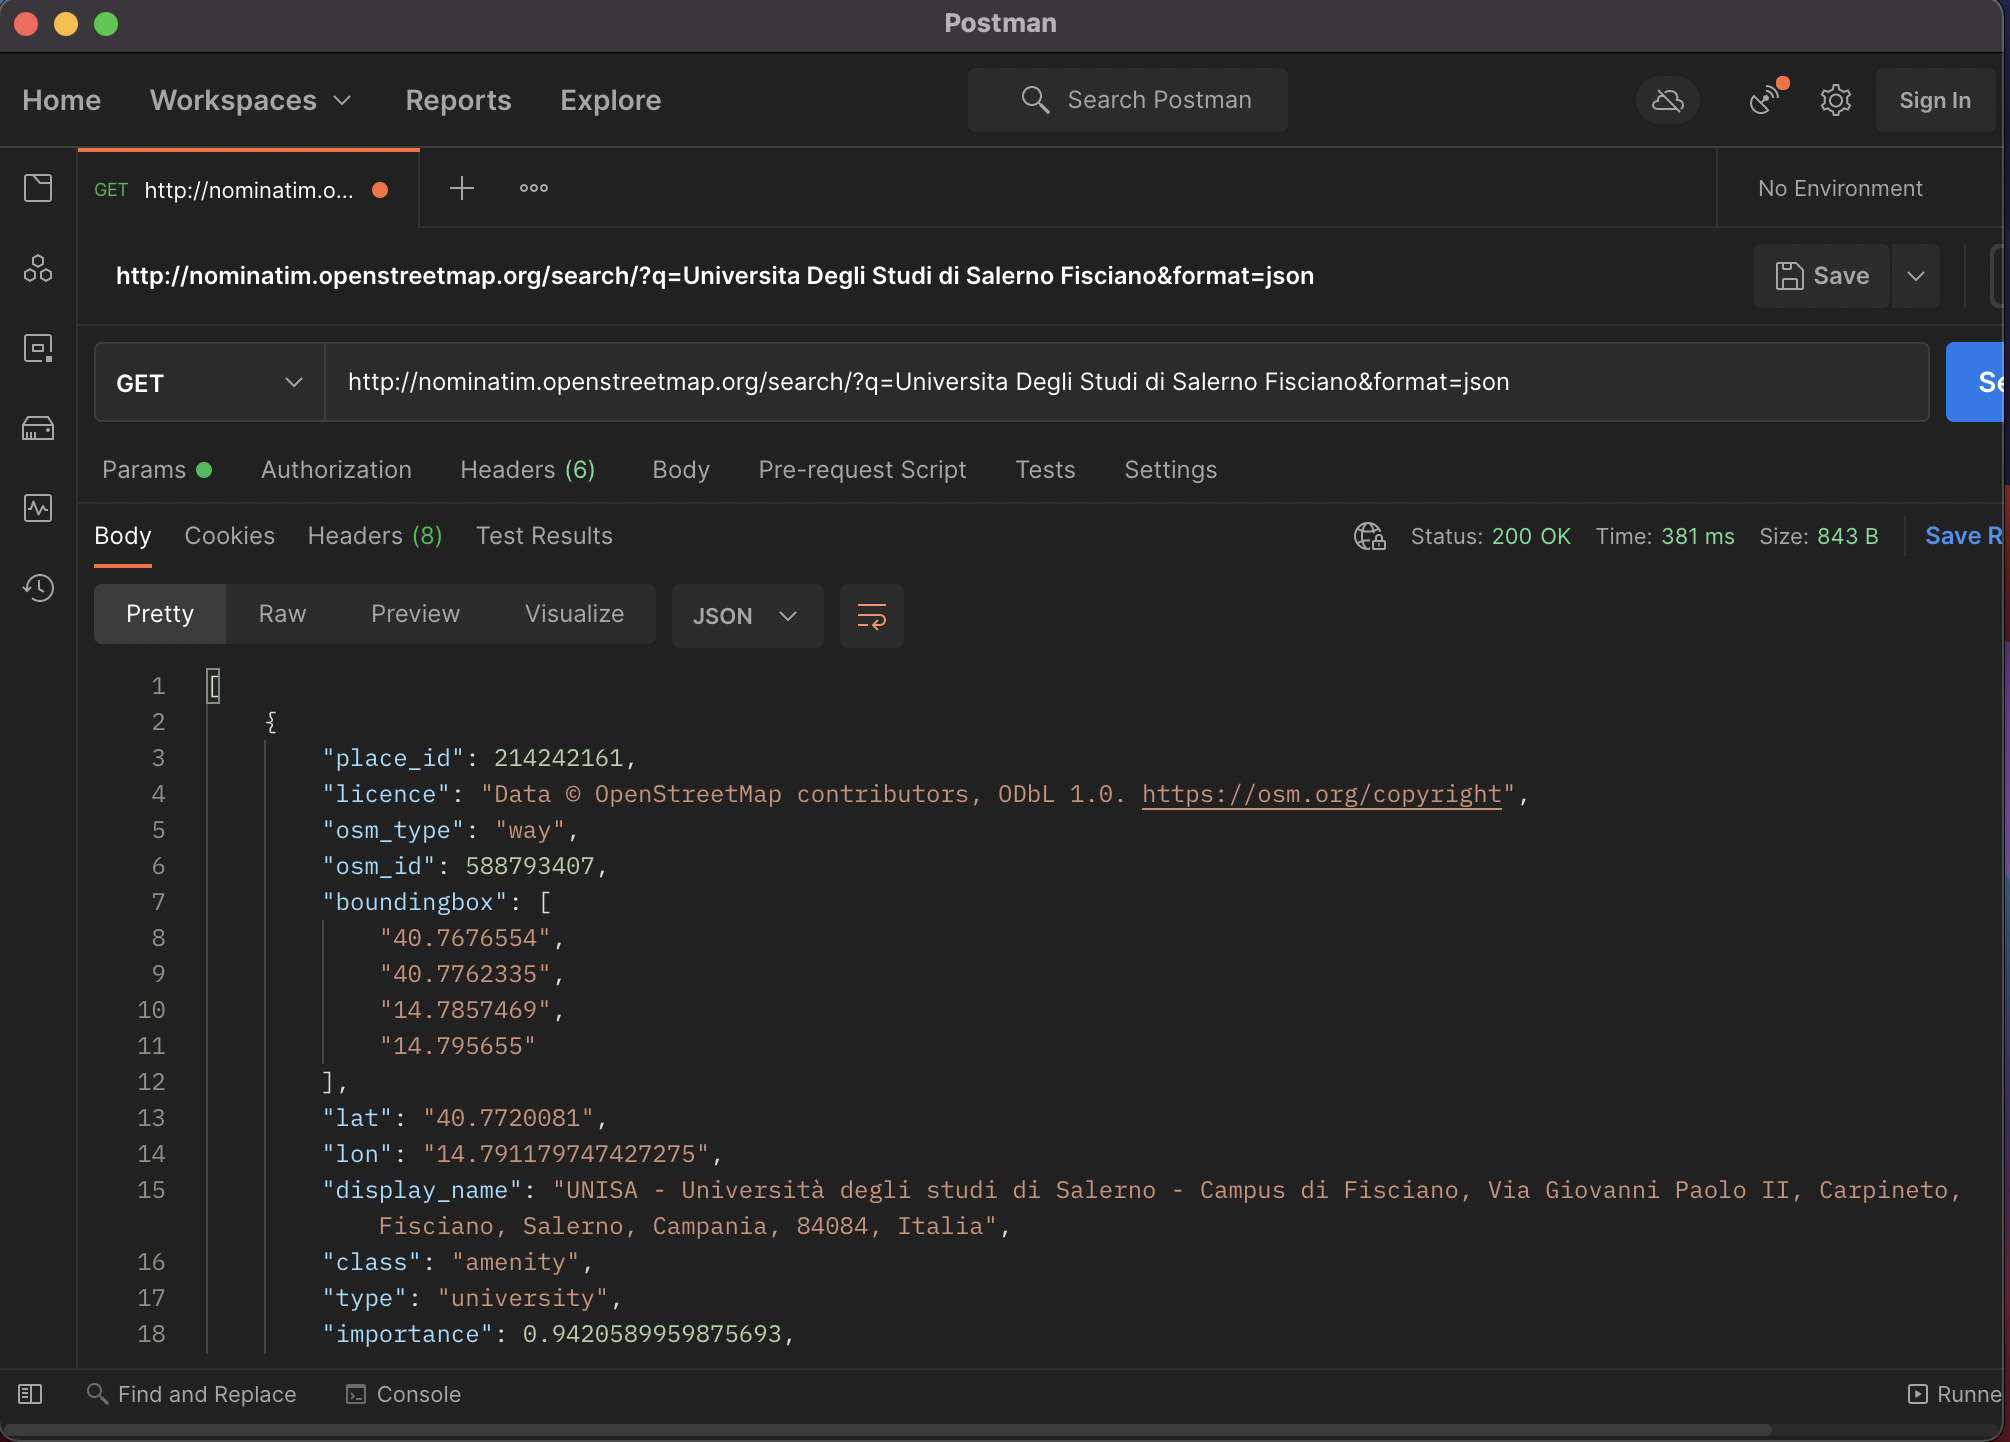
\includegraphics[width=\columnwidth]{search}
            \caption{Search}
            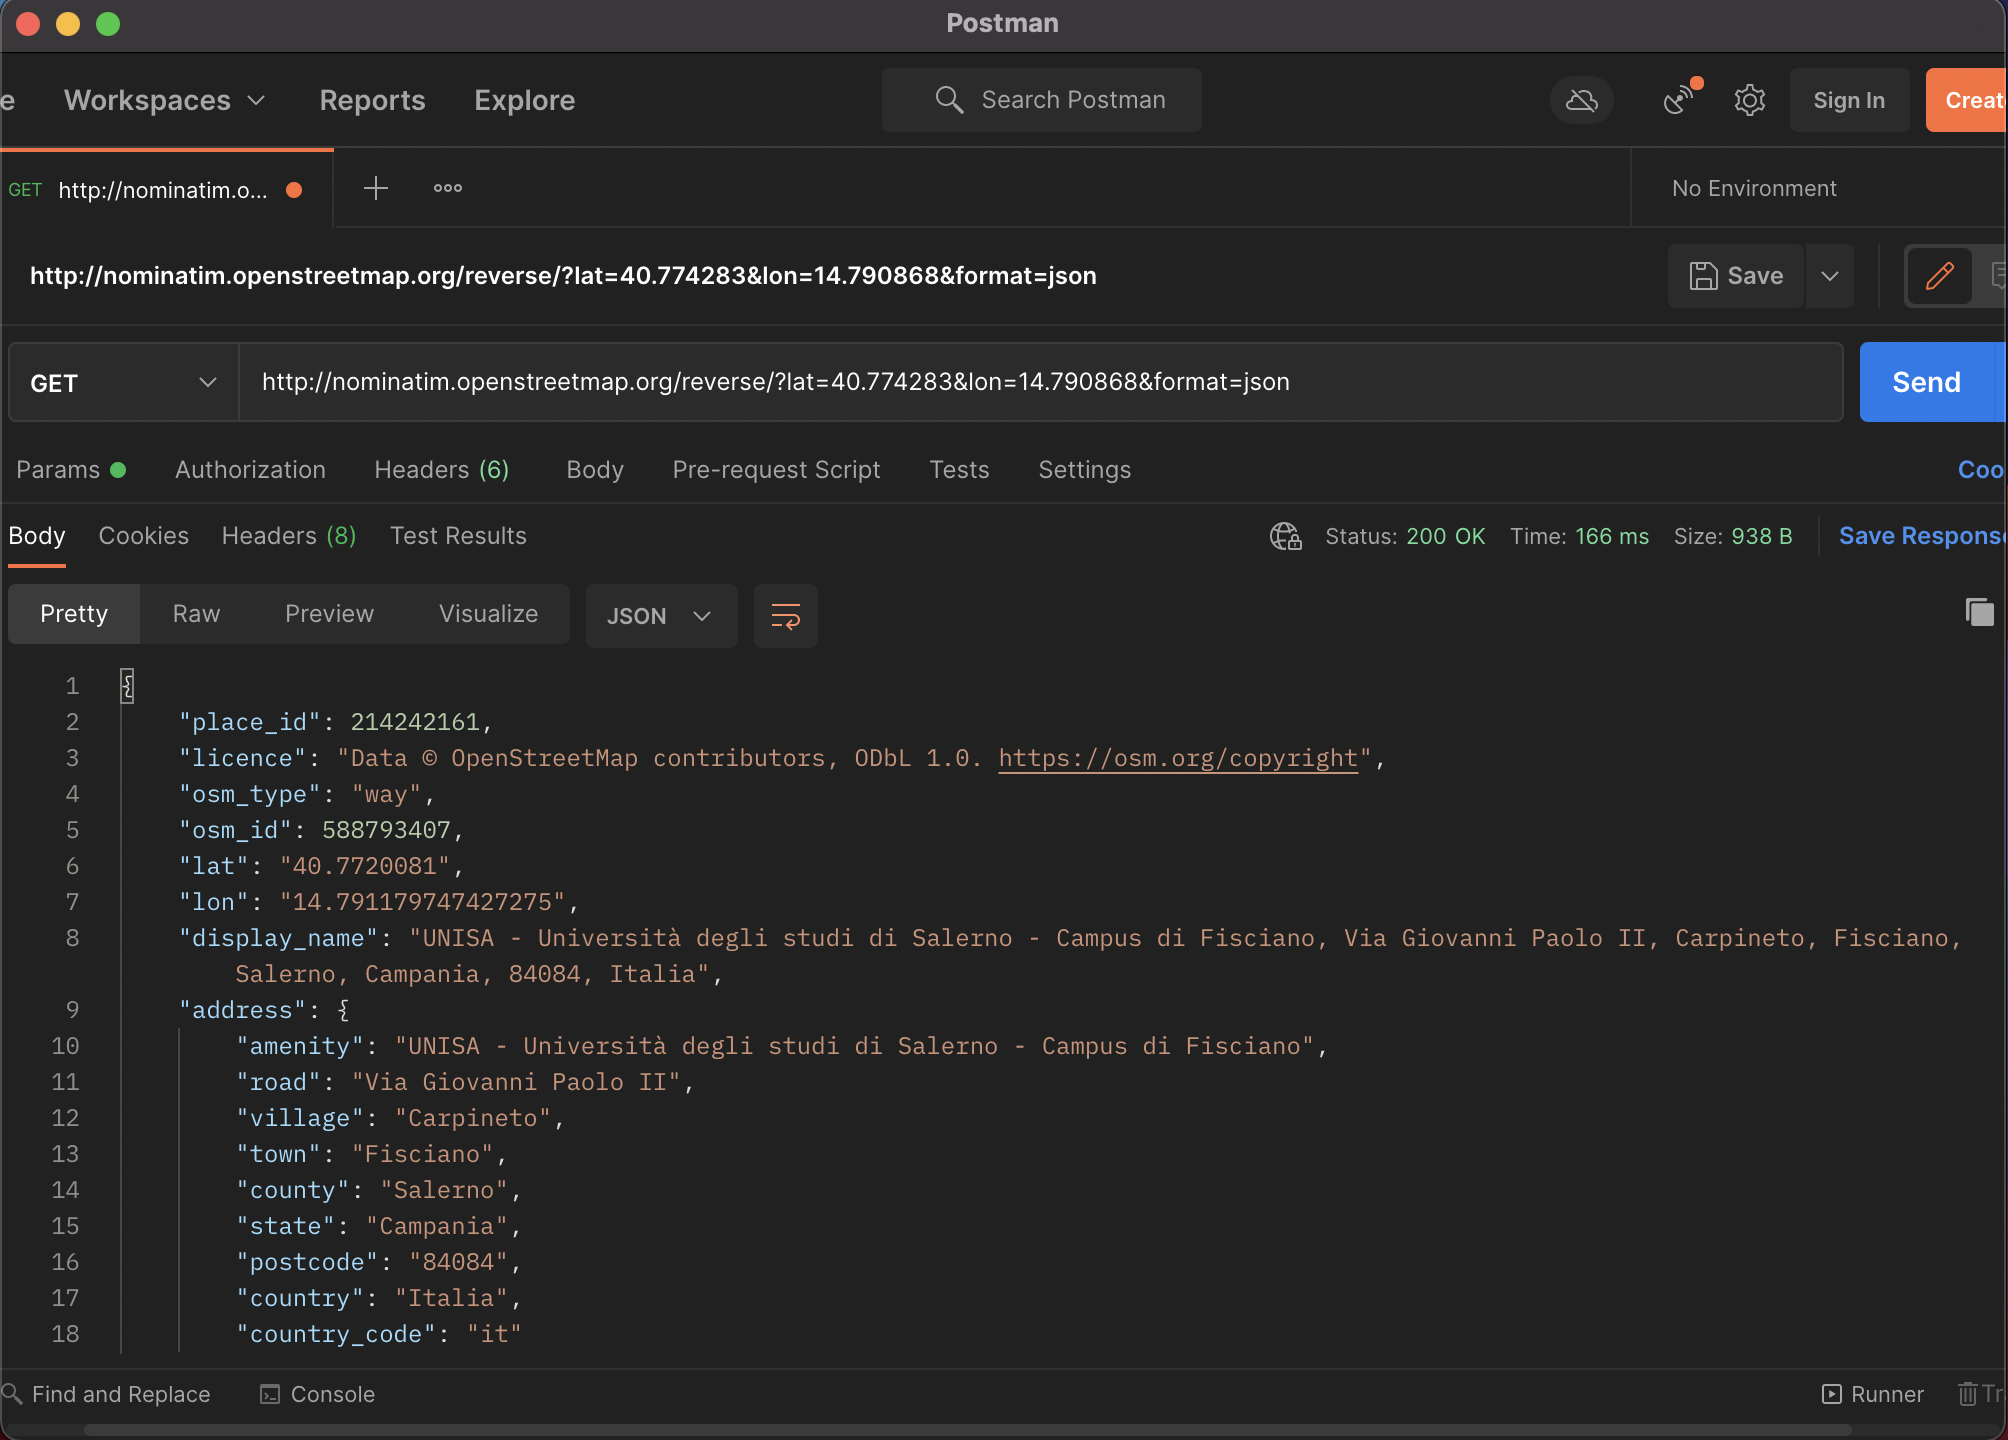
\includegraphics[width=\columnwidth]{reverse}
            \caption{Reverse}
        \end{figure}


        \newpage
        \subsubsection{Fonte dei dati utilizzati}
            Nominatim di per sé risulta essere solamente un servizio che permette di effettuare geocoding a partire da un dataset ma non ne fornisce nessuno out of the box. È stato quindi necessraio ottenere questi dati da entità terze. Un progetto che mette a disposizione pubblicamente questo tipo dei dati è chiamato Geofabrik, che ospita sui suoi server pacchetti organizzati per Stato o per Continente. Il formato di questi pacchetti risulta essere $.osm.pbf$, che è possibile importare all'interno di Nominatim attraverso un applicativo chiamato \textbf{osm2pgsql}. Quest'applicativo permette di importare dati organizzati secondo lo standard di OpenStreetMap all'interno di un database PostgreSQL/PostGIS. \\      